Les bases de données NoSQL possèdent une base commune qui est décrite dans cette partie. Chaque type de base de données NoSQL possède des spécificités, qui seront expliquées dans une partie dédiée.

\subsection{Les paires clé-valeur}
	La paire clé-valeur s'apparente comme la manière la plus simple de représenter tout type d'information. C'est pourquoi beaucoup de bases NoSQL partent du principe de base des paires clé-valeur afin de répondre à des besoins plus spécifiques. Le plus souvent  les bases de données NoSQL se contentent de spécifier un type pour la valeur de la paire (document, liste\dots). On peut faire le rapprochement avec une table d'une base de données relationnelle où la clé primaire permet d'identifier une ligne, qui peut être considérée comme une valeur.\\

	Le raisonnement de la paire clé-valeur est que les besoins d'accès aux données peuvent être simplifiés ainsi : à partir d'une clé de recherche, je veux obtenir une donnée complexe. Voici quelques exemples :
	\begin{itemize}
		\item Sur un réseau social, à partir d'un identifiant d'un utilisateur (la clé), je veux obtenir la liste de ses amis (la valeur) ;
		\item Dans un catalogue de livres, le numéro ISBN (la clé) donne accès à tous les détails sur le livre (la valeur) ;
		\item Sur un site de presse, la clé \texttt{article:42:comments} donne le nombre de commentaires postés sur l'article ayant l'identifiant 42.
	\end{itemize}
	\vspace{20px}

	La clé représente une information précise, simple et atomique alors que la valeur peut être complexe comme un tableau ou une liste, elle-même constituée de clés qui pointent sur des sous-valeurs.

\subsection{Recherche de simplicité et gestion des contraintes}
	Un des objectifs d'une paire clé-valeur est la simplicité. Il n'y a vraiment plus de notion de schéma de données dans un tel système. Chaque ligne peut être considérée comme étant complètement différente des autres, et s'il n'y a pas de système d'indexation secondaire, le seul accès valable est par la clé de la ligne.\\

	Le moteur de base de données qui n'utilise que des paires clé-valeur n'effectue aucune validation des données, que ce soit au niveau d'un schéma prédéfini ou de tous types de contraintes. C'est donc à l'application cliente de s'assurer que les données insérées dans la base de données sont bien cohérentes. Là où un SGBDR\footnote{SGBDR : Système de gestion de base de données} centralise la gestion des règles sur les données, un moteur NoSQL délègue cela au code client de chaque application utilisant la base de données.

\subsection{L'importance de la clé}
	La clé est le seul point d'entrée pour accéder à la valeur. Elle a donc une importance capitale. Dans un moteur NoSQL clé-valeur, par défaut, seule la clé est indexée.\\

	Souvent, cet index sur la clé est ce que l'on appelle un index \textit{clustered}. Les données sont ainsi physiquement ordonnées selon la clé entre les différentes machines (principe du \textit{sharding}), ce qui permet d'effectuer une recherche dichotomique rapide pour trouver la clé. Un index \textit{clustered} est illustré dans la figure~\ref{clusteredIndex}.

	\begin{figure}[H]
		\centering
		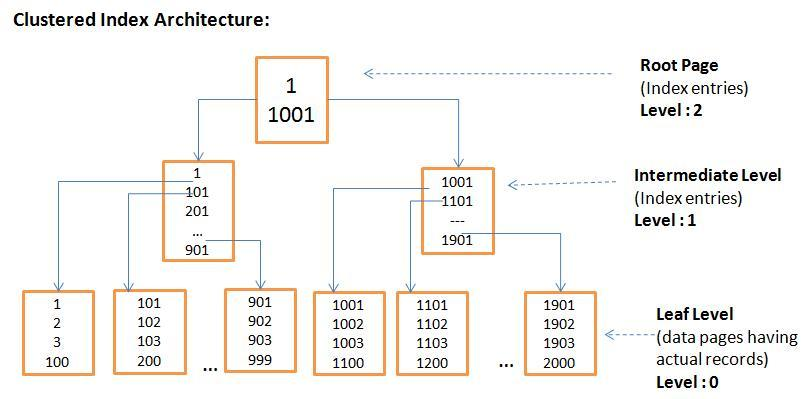
\includegraphics[width=0.9\textwidth]{images/clusteredIndex.jpg}
		\caption{Représentation d'un index \textit{clustered}.\cite{clusteredIndex}}
		\label{clusteredIndex}
	\end{figure}

	Bien évidemment les données peuvent être répliquées en plus d'être éparpillées sur plusieurs machines.
